\documentclass[12pt,a4paper]{article}
\usepackage[utf8]{inputenc}
\usepackage[spanish,es-tabla]{babel}
\usepackage{geometry}
\usepackage{graphicx}
\usepackage{multirow}
\usepackage{tabularx}
\usepackage{mathptmx}
\usepackage{fancyhdr}
\usepackage{array}
\usepackage[table]{xcolor}
\usepackage{titlesec}
\usepackage{setspace}
\usepackage{microtype}
\usepackage{lastpage}
\usepackage{booktabs}
\usepackage{enumitem}
\usepackage{amsmath}
\usepackage{amsfonts}
\usepackage{amssymb}
\usepackage{listings}

\lstset{
  basicstyle=\ttfamily\scriptsize,
  backgroundcolor=\color{gray!8},
  frame=single,
  breaklines=true,
  tabsize=2,
  showstringspaces=false
}

\graphicspath{{images/}{../images/}{./}}

\geometry{
    top=4.7cm,
    bottom=2.5cm,
    left=2.5cm,
    right=2.5cm,
    headheight=3.9cm,
    headsep=0.4cm
}

\setstretch{1.15}
\setlength{\parindent}{0pt}
\setlength{\parskip}{0.45em}
\setlength{\tabcolsep}{4pt}

\titleformat{\section}
  {\normalfont\fontsize{12}{14.5}\bfseries}{\thesection.}{0.6em}{\uppercase}
\titlespacing*{\section}
  {0pt}{1.8ex plus 0.4ex minus 0.2ex}{0.6ex plus 0.2ex}

\titleformat{\subsection}
  {\normalfont\fontsize{11.5}{13.5}\bfseries}{\thesubsection.}{0.5em}{}
\titlespacing*{\subsection}
  {0pt}{1.4ex plus 0.3ex minus 0.1ex}{0.4ex plus 0.1ex}

\titleformat{\subsubsection}
  {\normalfont\fontsize{10.5}{12.5}\bfseries\itshape}{\thesubsubsection.}{0.4em}{}
\titlespacing*{\subsubsection}
  {0pt}{1.1ex plus 0.2ex minus 0.1ex}{0.3ex plus 0.1ex}

\newcolumntype{Y}{>{\centering\arraybackslash}X}
\newcolumntype{L}{>{\raggedright\arraybackslash}X}
\newcolumntype{C}{>{\centering\arraybackslash}X}

\definecolor{headerred}{RGB}{180, 0, 0}
\definecolor{darkred}{RGB}{140, 0, 0}
\definecolor{lightgraybg}{RGB}{248, 248, 248}
\definecolor{tableheader}{RGB}{232, 238, 246}

\newcommand{\docCodigo}{TI-SIGE-ENT-S2-006}
\newcommand{\docVersion}{1.0}
\newcommand{\docProceso}{INGENIERÍA DE SOFTWARE / DEVOPS E INFRAESTRUCTURA}
\newcommand{\docElaboracion}{04/09/2026}
\newcommand{\docRevision}{PENDIENTE DE REVISIÓN}
\newcommand{\docTitulo}{ARQUITECTURA DE CONTENEDORES, ORQUESTACIÓN CON DOCKER COMPOSE Y DESPLIEGUE LOCAL}
\newcommand{\docOrganizacion}{FACULTAD DE INGENIERÍA EN SISTEMAS, ELECTRÓNICA E INDUSTRIAL}
\newcommand{\docSubOrganizacion}{CARRERA DE INGENIERÍA DE SOFTWARE}

\newcommand{\encabezadofrecuente}{%
    \renewcommand{\arraystretch}{1.15}%
    \noindent\makebox[\textwidth][c]{%
    \begin{tabularx}{\textwidth}{|>{\centering\arraybackslash}m{2.8cm}|Y|>{\centering\arraybackslash}m{4.8cm}|}
        \hline
        \multirow{4}{2.8cm}{\centering\raisebox{-1.15cm}{
\includegraphics[width=2.5cm,height=2.0cm,keepaspectratio]{images/logo.png}}}
        & \textbf{\fontsize{9}{11}\selectfont \docOrganizacion} 
        & \textbf{\fontsize{8}{10}\selectfont CÓDIGO:} \fontsize{8}{10}\selectfont \docCodigo \\
        \cline{3-3}
        & \textbf{\fontsize{8.5}{10.5}\selectfont \docSubOrganizacion} 
        & \textbf{\fontsize{8}{10}\selectfont VERSIÓN:} \fontsize{8}{10}\selectfont \docVersion \\
        \cline{2-3}
        & \textbf{\fontsize{8}{10}\selectfont PROCESO:} \fontsize{8}{10}\selectfont \docProceso 
        & \textbf{\fontsize{8}{10}\selectfont ELABORACIÓN:} \fontsize{8}{10}\selectfont \docElaboracion \\
        \cline{2-3}
        & \textbf{\fontsize{8.5}{10.5}\selectfont \docTitulo} 
        & \textbf{\fontsize{8}{10}\selectfont ÚLTIMA REVISIÓN:} \fontsize{8}{10}\selectfont \textbf{\textcolor{darkred}{\docRevision}} \\
        \hline
    \end{tabularx}%
    }%
}

\pagestyle{fancy}
\fancyhf{}
\fancyhead[C]{\encabezadofrecuente}
\fancyfoot[C]{\fontsize{10}{12}\selectfont Página \thepage\ de \pageref{LastPage}}
\renewcommand{\headrulewidth}{0pt}

\begin{document}

\section{Título}
\textbf{Denominación del Entregable:} Configuración de Infraestructura como Código (IaC), Contenedores y Docker Compose (EDT 2.6)

\vspace{0.15cm}
\noindent
\textbf{Ficha Técnica de Identificación:}
\begin{itemize}[leftmargin=1.5em, itemsep=1.5pt, topsep=1.5pt]
    \item \textbf{Código Documental:} \docCodigo \quad | \quad \textbf{Versión:} \docVersion
    \item \textbf{Institución:} Universidad Técnica de Ambato (UTA) -- FISEI
    \item \textbf{Carrera:} Ingeniería de Software (Séptimo Semestre "A")
    \item \textbf{Módulo Académico:} Gestión de Proyectos de Software
    \item \textbf{Docente Tutor:} Ing. Paulo Torres
    \item \textbf{Fecha de Elaboración:} \docElaboracion \quad | \quad \textbf{Estado:} \textbf{\textcolor{darkred}{En Elaboración / Pendiente de Revisión}}
    \item \textbf{Período de Ejecución:} Semana 2 (02/09/2026 al 04/09/2026)
    \item \textbf{Responsables:} Steeven Toala (Líder / Arquitecto) y Nixon Hurtado (Backend / DBA)
\end{itemize}

\section{Introducción}
Para garantizar reproducibilidad en los entornos de desarrollo, pruebas y producción sin incurrir en costos de licencias comerciales ni saturar los recursos de hardware, el sistema \textbf{SIGE} implementa una arquitectura eficiente y desacoplada mediante \textbf{Docker Compose}: servicios locales contenerizados (PostgreSQL 16, MinIO, LanguageTool, Backend .NET 9, Frontend React 19) e inferencia semántica delegada a la \textbf{API de Google Gemini (Gemini 1.5 / 2.0 Flash)} a través de HTTPS sin costo de GPU local.

\section{Objetivo}

\subsection{Objetivo General}
Diseñar, configurar y orquestar la arquitectura de contenedores Docker locales para el ecosistema completo de SIGE, asegurando reproducibilidad y despliegue automatizado en la FISEI UTA.

\subsection{Objetivos Específicos}
\begin{enumerate}[leftmargin=1.5em, itemsep=2pt, topsep=2pt]
    \item Configurar los 6 servicios del \texttt{docker-compose.yml} (PostgreSQL, MinIO, MinIO-Init, LanguageTool, Backend y Frontend).
    \item Establecer las redes virtuales internas y políticas de persistencia en volúmenes nombrados.
    \item Parametrizar las variables de entorno y definir los endpoints de Health Check.
\end{enumerate}

\section{Alcance}

\subsection{Límites del Despliegue (In-Scope)}
\begin{itemize}[leftmargin=1.5em, itemsep=2pt]
    \item Orquestación local para desarrollo y producción On-Premise en un host con Docker Engine 24+.
\end{itemize}

\subsection{Exclusiones (Out-of-Scope)}
\begin{itemize}[leftmargin=1.5em, itemsep=2pt]
    \item Clústeres Kubernetes distribuidos en múltiples nodos de nubes comerciales de pago.
\end{itemize}

\section{Definiciones}
\begin{itemize}[leftmargin=1.5em, itemsep=2pt]
    \item \textbf{Docker Compose:} Herramienta para definir y ejecutar aplicaciones multi-contenedor mediante archivos YAML.
    \item \textbf{Named Volume:} Mecanismo de persistencia de datos gestionado por Docker independiente del ciclo de vida del contenedor.
    \item \textbf{Healthcheck:} Instrucción que comprueba periódicamente el estado operativo interno de un servicio.
\end{itemize}

\section{Responsabilidades}
\begin{table}[htbp]
\centering
\small
\begin{tabularx}{\textwidth}{|>{\hsize=0.65\hsize\bfseries}X|>{\hsize=0.85\hsize}X|>{\hsize=1.5\hsize}X|}
    \hline
    \rowcolor{tableheader}
    Integrante & Rol en el Entregable & Responsabilidad Específica \\
    \hline
    Steeven Toala & Líder / Arquitecto & Diseño de Dockerfiles, archivo \texttt{docker-compose.yml} y configuración de redes. \\
    \hline
    Nixon Hurtado & Backend / DBA & Configuración del contenedor de PostgreSQL 16 y persistencia de volúmenes. \\
    \hline
    Ing. Paulo Torres & Docente Tutor & Validación y prueba del despliegue en un único comando. \\
    \hline
\end{tabularx}
\caption{Matriz de Responsabilidades del Entregable EDT 2.6.}
\end{table}

\section{Normativa Legal y Técnica}
\begin{itemize}[leftmargin=1.5em, itemsep=2pt]
    \item \textbf{Open Container Initiative (OCI) Image Specification v1.1.}
    \item \textbf{CIS Docker Benchmark v1.6.0:} Guía de endurecimiento de seguridad en contenedores.
\end{itemize}

\section{Método, Políticas y Contenidos}
La topología de servicios contenerizados conectados bajo la red puente \texttt{sige-network} se estructura de la siguiente manera:

\begin{itemize}[leftmargin=1.5em, itemsep=2pt]
    \item \textbf{Servicios Locales Contenerizados:} Base de datos relacional (\textbf{PostgreSQL 16}), almacenamiento de objetos S3 (\textbf{MinIO}), corrector ortográfico/gramatical local de alta velocidad (\textbf{LanguageTool}), backend (\textbf{ASP.NET Core .NET 9}) y cliente web (\textbf{React 19 + Nginx}).
    \item \textbf{Asistencia Semántica de Inteligencia Artificial:} En lugar de ejecutar un contenedor local pesado de Ollama (que requeriría descargar modelos de varios gigabytes y consumir entre 8 y 16 GB de RAM con soporte GPU inviable en infraestructura económica), la inferencia semántica para redacción institucional se delega a la \textbf{API de Google Gemini (Gemini 1.5 / 2.0 Flash)} a través de peticiones seguras HTTPS (REST API), optimizando la infraestructura local a cero sobrecosto de hardware.
\end{itemize}

\begin{figure}[htbp]
    \centering
    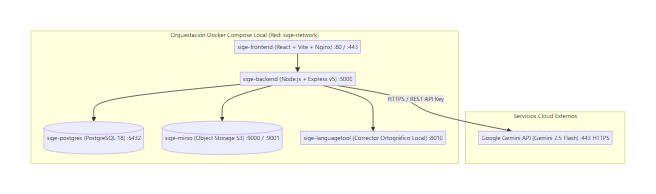
\includegraphics[width=0.82\textwidth,height=5.2cm,keepaspectratio]{images/s2_06_docker_compose.png}
    \caption{Arquitectura de Contenedores y Mapeo de Puertos en Docker Compose.}
    \label{fig:s2_06_docker}
\end{figure}

\section{Descripción de actividades}

\subsection{Especificación del Archivo \texttt{docker-compose.yml}}
\begin{lstlisting}[language=XML]
version: '3.8'

services:
  # 1. Base de Datos Relacional PostgreSQL 16
  sige-postgres:
    image: postgres:16-alpine
    container_name: sige-postgres
    restart: unless-stopped
    environment:
      POSTGRES_DB: sige_db
      POSTGRES_USER: sige_admin
      POSTGRES_PASSWORD: SigeSecurePassword2026!
    ports:
      - "5432:5432"
    volumes:
      - postgres_data:/var/lib/postgresql/data
    networks:
      - sige-network
    healthcheck:
      test: ["CMD-SHELL", "pg_isready -U sige_admin -d sige_db"]
      interval: 10s
      timeout: 5s
      retries: 5

  # 2. Servidor de Objetos MinIO (Almacenamiento Seguro S3)
  sige-minio:
    image: minio/minio:RELEASE.2024-05-10T01-41-38Z
    container_name: sige-minio
    restart: unless-stopped
    command: server /data --console-address ":9001"
    environment:
      MINIO_ROOT_USER: sige_minio_admin
      MINIO_ROOT_PASSWORD: SigeMinioSecretKey2026!
    ports:
      - "9000:9000"   # API S3 Endpoint
      - "9001:9001"   # Consola Web de Administracion
    volumes:
      - minio_data:/data
    networks:
      - sige-network

  # 3. Inicializador de Bucket MinIO (Crea el bucket de evidencias automaticamente)
  sige-minio-init:
    image: minio/mc:latest
    container_name: sige-minio-init
    depends_on:
      - sige-minio
    entrypoint: >
      /bin/sh -c "
      until (/usr/bin/mc config host add sigeMinio http://sige-minio:9000 sige_minio_admin SigeMinioSecretKey2026!) do echo 'Esperando a MinIO...' && sleep 2; done;
      /usr/bin/mc mb sigeMinio/sige-evidencias-bucket --ignore-existing;
      /usr/bin/mc anonymous set download sigeMinio/sige-evidencias-bucket;
      exit 0;
      "
    networks:
      - sige-network

  # 4. Servidor Local LanguageTool (Corrector Ortografico en Espanol)
  sige-languagetool:
    image: erikvl87/languagetool:latest
    container_name: sige-languagetool
    restart: unless-stopped
    environment:
      langtool_languageModel: "/ngrams"
      Java_Xms: "512m"
      Java_Xmx: "1g"
    ports:
      - "8010:8010"
    networks:
      - sige-network

  # 5. Backend ASP.NET Core (.NET 9 Web API)
  sige-backend:
    build:
      context: ./src
      dockerfile: SIGE.WebAPI/Dockerfile
    container_name: sige-backend
    restart: unless-stopped
    depends_on:
      sige-postgres:
        condition: service_healthy
      sige-minio:
        condition: service_started
      sige-languagetool:
        condition: service_started
    environment:
      - ASPNETCORE_ENVIRONMENT=Development
      - ConnectionStrings__DefaultConnection=Host=sige-postgres;Port=5432;Database=sige_db;Username=sige_admin;Password=SigeSecurePassword2026!;
      - MinIO__Endpoint=sige-minio:9000
      - MinIO__AccessKey=sige_minio_admin
      - MinIO__SecretKey=SigeMinioSecretKey2026!
      - MinIO__BucketName=sige-evidencias-bucket
      - MinIO__UseSSL=false
      - LanguageTool__BaseUrl=http://sige-languagetool:8010
      - Gemini__ApiKey=${GEMINI_API_KEY}
      - Gemini__Model=gemini-1.5-flash
    ports:
      - "5000:8080"
    networks:
      - sige-network

  # 6. Frontend React 19 + Nginx
  sige-frontend:
    build:
      context: ./src/SIGE.ClientApp
      dockerfile: Dockerfile
    container_name: sige-frontend
    restart: unless-stopped
    depends_on:
      - sige-backend
    ports:
      - "80:80"
    networks:
      - sige-network

networks:
  sige-network:
    driver: bridge

volumes:
  postgres_data:
    driver: local
  minio_data:
    driver: local
\end{lstlisting}

\subsection{Comandos de Despliegue y Verificación Local}

\subsection{Inicio de Servicios}
\begin{lstlisting}[language=bash]
# 1. Clonar el repositorio y posicionarse en la raiz
cd d:/2Proyectos/GESTION_DE_PROYECTOS_DE_SOFTWARE/FISEI_Project

# 2. Levantar todos los contenedores en segundo plano
docker compose up -d

# 3. Verificar estado operativo de los servicios
docker compose ps
\end{lstlisting}

\subsection{Endpoints de Verificación de Salud (Health Checks)}
\begin{itemize}[leftmargin=1.5em, itemsep=2pt]
    \item \textbf{Frontend Web:} \texttt{http://localhost:80}
    \item \textbf{Swagger Web API:} \texttt{http://localhost:5000/swagger}
    \item \textbf{Consola MinIO:} \texttt{http://localhost:9001} (User: \texttt{sige\_minio\_admin} / Pass: \texttt{SigeMinioSecretKey2026!})
    \item \textbf{API LanguageTool:} \texttt{http://localhost:8010/v2/check?text=Hola\%20mundo\&language=es}
    \item \textbf{Asistente Gemini AI:} Conectividad HTTPS directa con \texttt{https://generativelanguage.googleapis.com} (verificable vía \texttt{/api/ia/status} en backend con API Key institucional).
\end{itemize}

\vspace{0.3cm}

% =============================================================
% FIRMAS DE RESPONSABILIDAD
% =============================================================
\section{Firmas de Responsabilidad}

\noindent
\renewcommand{\arraystretch}{1.2}
\begin{tabularx}{\textwidth}{|>{\raggedright\arraybackslash}m{2.9cm}|>{\raggedright\arraybackslash}X|>{\centering\arraybackslash}m{4.6cm}|>{\centering\arraybackslash}m{2.3cm}|}
    \hline
    \rowcolor{headerred}
    \textcolor{white}{\textbf{ACCIÓN}} & \textcolor{white}{\textbf{NOMBRE Y CARGO}} & \textcolor{white}{\textbf{FIRMA}} & \textcolor{white}{\textbf{FECHA}} \\
    \hline
    \textbf{Elaborado por:} & Steeven Toala\newline \textit{Líder de Proyecto / Arquitecto Software} & \parbox[c]{4.4cm}{\centering\vspace{4pt}
\includegraphics[height=1.5cm,width=4.0cm,keepaspectratio]{images/firma_steveen.png}\vspace{4pt}} & 04/09/2026 \\
    \hline
    \textbf{Revisado por:} & Steeven Toala\newline \textit{Líder de Proyecto / Arquitecto Software} & \parbox[c]{4.4cm}{\centering\vspace{10pt}\textbf{\textcolor{gray!80}{\scriptsize [ PENDIENTE DE REVISIÓN ]}}\vspace{10pt}} & \textbf{\textcolor{gray!90}{Pendiente}} \\
    \hline
    \textbf{Aprobado por:} & Ing. Paulo Torres\newline \textit{Docente Tutor - Gestión Proyectos Software} & \parbox[c]{4.4cm}{\centering\vspace{10pt}\textbf{\textcolor{gray!80}{\scriptsize [ PENDIENTE DE APROBACIÓN ]}}\vspace{10pt}} & \textbf{\textcolor{gray!90}{Pendiente}} \\
    \hline
\end{tabularx}

\vspace{0.4cm}

% =============================================================
% CONTROL DE CAMBIOS
% =============================================================
\section{Control de Cambios}

\noindent
\renewcommand{\arraystretch}{1.2}
\begin{tabularx}{\textwidth}{|>{\hsize=0.45\hsize\centering\arraybackslash}X|>{\hsize=1.55\hsize\raggedright\arraybackslash}X|>{\hsize=1.2\hsize\raggedright\arraybackslash}X|>{\hsize=0.8\hsize\centering\arraybackslash}X|}
    \hline
    \rowcolor{gray!20}
    \textbf{Versión} & \textbf{Descripción del cambio} & \textbf{Responsable del cambio} & \textbf{Fecha de aprobación} \\
    \hline
    1.0 & Configuración de docker-compose.yml con los 6 servicios y comandos de verificación / Pendiente de revisión & Steeven Toala & \textbf{\textcolor{gray!90}{Pendiente de Revisión}} \\
    \hline
\end{tabularx}

\vspace{0.4cm}

\section{Anexos}
\subsection*{Anexo 1: Script de Inicialización de Redes y Volúmenes de Docker}
Comandos \texttt{docker volume inspect} y políticas de reinicio automático ante fallos de contenedor.

\end{document}
